\documentclass[en,hazy,blue,screen,14pt]{elegantnote}
\usepackage[T1]{fontenc}
\usepackage[latin9]{inputenc}
\usepackage{babel}
\usepackage{float}
\usepackage{textcomp}
\usepackage{amsmath,amsfonts,amssymb}
\usepackage{amsthm}
\usepackage{graphicx}
%\usepackage[ruled,vlined]{algorithm2e}
\PassOptionsToPackage{normalem}{ulem}
\usepackage{ulem}
\usepackage{mathtools}
\usepackage{url}
\usepackage{hyperref}
\usepackage{algorithm, algpseudocode}

\renewcommand\qedsymbol{$\blacksquare$}
\DeclarePairedDelimiter{\ceil}{\lceil}{\rceil}
\newcommand\tab[1][1cm]{\hspace*{#1}}
\newenvironment{claim}[1]{\par\noindent\underline{Claim:}\space#1}{}
\newenvironment{claimproof}[1]{\par\noindent\underline{Proof:}\space#1}{\hfill $\blacksquare$}
\renewcommand{\algorithmicrequire}{\textbf{Input:}}
\renewcommand{\algorithmicensure}{\textbf{Output:}}

\title{Class Notes\\CIS 502 Analysis of Algorithm\\7-NP Completeness}
\author{Da Kuang}
\institute{University of Pennsylvania}
% \version{1.00}
\date{}

\begin{document}

\maketitle
\newpage
% \input{}
\section{Polynomial Time}
A holistic view of efficiency

We have been seeking to design efficient algorithms but have not defined ``efficiency''!

Algorithms have running times that grow with the size of the input. If algorithm are to be scalable, this growth rate should not be too fast. \textbf{A growth rate that is polynomial in the input size is considered efficient}, and anything faster than a polynomial is considered inefficient (for several good reasons)

What do we mean by polynomial time?
\begin{itemize}
	\item The running time is $O(n^c)$ for some constant $c$.
	\item Examples: $O(n^3)$ and $O(n \log n)$ are poly-time. $O(2^n)$, $O(n^{\log n})$ and $O(n!)$ are not.
\end{itemize}

Most problems of interest have exponentially more possibilities to be considered. For example, for the activity selection problem, we need to implicitly consider all $2^n$ subsets of activities. If we really calculate all of them, then we could have an exponential time algorithm. Coming up with a polynomial time algorithm means that we have developed some insight into the problem that allows us to avoid this brute force search.

Polynomial time is also an incredibly \textbf{robust} class; if we consider any other reasonable model of computation, and any other reasonable way of encoding the input, an algorithm that was polynomial time will stay polynomial time. 

If you design a function that runs in polynomial time, then polynomially more invocations of this function also take polynomial time. This is because polynomials are \textbf{closed under composition}.

\subsection{Further Discussion: Objection}
There is a possible objection: an algorithm that runs in time $n^{100}$ is poly-time but hardly scalable; it is already in feasible on inputs of size $2$.

It is true. But We do not know any natural problem for which the poly-time algorithm runs in time $n^{100}$. Even if the first poly-time algorithm for the problem is impractical, it already brings some insights into the problem and the running time can be quickly improved.

\subsection{Toss a Coin}
We actually go a little further than polynomial time in what we consider efficient: we allow algorithms to toss coins, and even a randomized algorithm that runs in polynomial time is considered efficient.

\subsection{Decision Problems}
When we study polynomial time algorithms and beyond, we will restrict ourselves to \textbf{decision problems}, meaning problems where the answer on each instance is YES or NO (also 1 or 0).

Many problems we have studied are ``search problems'', not decision problems. For example, find the minimum spanning tree, find the optimal Huffman encoding, etc.

However, for each of these problems, there is a closely related decision problem. If we can solve this related decision problem in polynomial time, then we can solve the search problem in polynomial time.

For example, given a weighted, undirected graph and a number $K$, is there an MST whose weight is $\le K$? This is the decision problem closely related to MST search.

Another example, given input to Huffman, and a real number $\alpha$, is there a code with average length at most $\alpha$.

\subsection{Decision vs. Search}
How does solving the decision version of MST help find MST?

Suppose we are given a black box $B$ that takes as input $(G, K)$, and outputs YES if $G$ has an MST of weight at most $K$ and NO otherwise.

Assume the graph weights and $K$ are integers.

We check $B(G, K)$ for $K = \frac{\sum_{e \in G} w(e)}{2}$:
\begin{itemize}
	\item If YES, we binary search downwards
	\item If NO, we binary search upwards to arrive at $K = $  weight of MST.
\end{itemize}

We fix this $K$,
\begin{itemize}
	\item We successively remove edges from $G$ and see if new graph still has MST of weight $K$.
	\item If it does not, we put back the edge we remove; it is needed in the MST.
\end{itemize}

At the end, we will have found the MST in polynomial many calls to $B$.

\subsection{P}
P (read as ``polynomial time'') is the class of decision problems for which there is a polynomial time algorithm.

A class of problem defined by a resource constraint (such as a constraint on running time or space) is called a complexity class. P is one of the most important complexity class.

When encountering a new computational problem, one of the first question you should ask yourself is: 

"\textbf{is this problem in $P$?}"

For this section of the course, we will be less concerned with getting the best possible running time. We will be happy as long as we can tell it is in $P$ or not.














\section{Non-Deterministic Polynomial Time (NP)}
\subsection{Beyond P}
We have painted a rosy picture for algorithmic solutions, by picking problems that have polynomial time solutions and designing poly-time algorithm for them. However, the problems you will encounter in the real world and in your careers will not have such efficient solutions. 

Many of these decision problems share an interesting feature: if you are given a YES instance of the problem, and a ``solution'' to this YES instance, then you can verify that this is a YES instance in polynomial time.

For example,
\begin{itemize}
	\item A Hamilton Cycle (HC) in a graph is a simple cycle that passes through all vertices without hitting any vertex twice.
	\item The HC decision problem is: given a graph $G$, does it have a Hamilton Cycle?
	\item We believe it is a hard problem, but if a certain $G$ is a YES instance, and we were also given the Hamilton cycle itself, we could efficiently verify this and confirm that it is a YES instance.
\end{itemize}

The verification algorithm is given two inputs: $G$ and a proposed Hamilton cycle $v_1, v_2, \cdots, v_n, v_1$.
\begin{itemize}
	\item It first checks that the cycle is simple and passes through all vertices, by checking that every vertex occurs and that no vertex occurs twice (expect the start and end vertices).
	\item Next, it confirms that each $(v_i, v_{i+1})$ for $i = 1, 2, \cdots, n-1$ is an edge in $G$. It also checks that $(v_n, v_1)$ is an edge.
	\item Now it is convinced that $G$ is a YES instance.
\end{itemize}
Note that we are not saying that we can efficiently find the Hamilton Cycle! We are just saying that, given the cycle, we can verify that $G$ is a YES instance.

\subsection{``NP''}
Many difficult problems you will encounter share this property: for YES instance, there is a ``solution'' that can be easily verified. Such a solution is called many names: certificate, proof, or witness.

A decision problem $\pi$ is in \textbf{NP} (read as ``non-deterministic polynomial time'') if there is a polynomial time verification algorithm $V$ such that:
\begin{itemize}
	\item If $x$ if a YES instance of $\pi$, there exists a certificate $y$ whose length is polynomial in $|x|$ such that $V(x, y)$ accepts.
	\item If $x$ is a NO instance of $\pi$, then for any string $y$, $V(x, y)$ rejects.
\end{itemize}

Again, note that we are not talking about computing $y$ efficiently. In fact, we believe that, for many problems in \textbf{NP}, there is no efficient way to compute $y$.
\subsection{Examples}
\subsubsection{Maximum Clique Problem}
Given a graph $G$ and a number $K$, are there $K$ vertices in $G$ that are all pairwise adjacent? Such group of vertices are called clique.

This kind of problem is useful for finding groups of mutual friends in social networks.

Certificate: the $K$ vertices that form the clique. Verification is straightforward.

\begin{figure}[H]
	\centering
	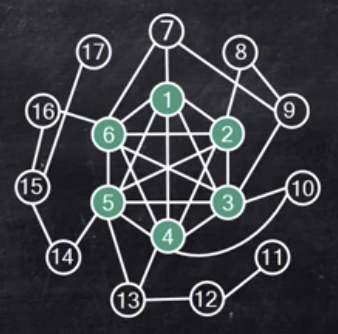
\includegraphics[width=0.3\textwidth]{fig/max-clique-2.png}
\end{figure}

\subsubsection{3-Coloring Problem}
Given a graph $G$, can we assign 3 colors to its vertices so that any pair of adjacent vertices have different colors?

This kind of problem is useful for allocating frequencies to radio stations to avoid interference, deciding which activities to schedule in which rooms, or allocating registers to variables in a program.

Certificate: the colors of the vertices. Easy to verify coloring by examining all edges.

\begin{figure}[H]
	\centering
	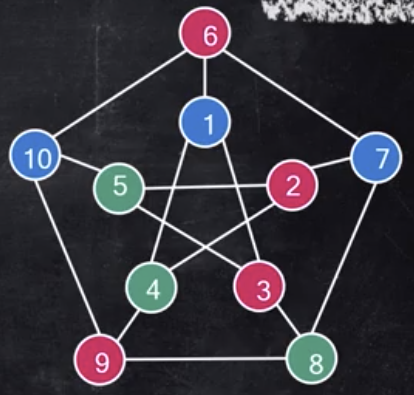
\includegraphics[width=0.3\textwidth]{fig/3-color.png}
\end{figure}

\subsubsection{Partition Problem}
Given $n$ numbers, can they be partitioned into 2 sets such that the sums of the numbers in the sets are equal?

Certificate: the actual partition into two sets. Easy to verify that each part adds to the same total.

\begin{figure}[H]
	\centering
	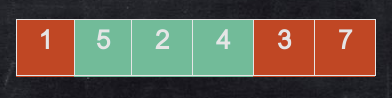
\includegraphics[width=0.3\textwidth]{fig/partition.png}
\end{figure}

\subsection{Asymetry In Definitions of P and NP}
For a problem $\pi$ to be in NP, only the YES instances have certificates accepted by the verifier. There aren't any certificates for the NO instance. So if you are given an instance of the clique problem $(G, K)$, we do not know any short certificate that will demonstrate that $G$ does not have a clique of size $K$.

Example: an integer $N$ is composite if it has a factor $p$: $1 < p < N$.
\begin{itemize}
	\item Composites are in NP.
	\item Given a YES instance i.e. a composite number, a certificate demonstrating that $N$ is composite is a non-trivial factor $p$.
	\item It is not immediately clear that NO instance are also efficiently verifiable.
	\item Given $N$ that is not a composite, i.e. a prime number, what would a certificate be?
	\item In this case, it turns out that there are certificates for primality but understanding how they work requires some knowledge of abstract algebra.
\end{itemize}

\subsection{``Co-NP''}
Given the asymmetry we observed, we could define a complexity class of problems for which NO instances can be efficiently verified. This is the class \textbf{Co-NP}.

The complement of a decision problem $\pi$ is the problem $\pi'$ defined as: $x$ is a YES instance of $\pi$ if and only if it is a NO instance of $\pi'$.

A problem $\pi'$ is in Co-NP if and only if its complement $\pi$ is in NP.


\subsection{Turing Machine Definition of NP}
A problem is in NP if there exists a non-deterministic TM that can decide if $x$ is a YES or NO instance in polynomial time.














\section{Reduction}
Settling the P versus. NP question will have huge ramifications. If P=NP, tens of thousands of real world problems will have efficient solutions. This will have enormous implications for business, medicine, science, etc. Automation could replace human ingenuity in many more spheres. While on the down side, cryptography will no longer be possible.

Most researchers in the field do not believe that P=NP. But how do we go about finding the answer?

\subsection{One Approach}
Identify the ``hardest'' problems in NP, such that solving any one of them in polynomial would show that $\text{P} = \text{NP}$. Try your best to find a polynomial time algorithm for one such problem. 

But how do we identify the hardest problems in NP?

Attempted definition: a problem $\pi$ is ``a hardest problem'' in NP if, given an efficient algorithm to solve $\pi$, you can use it (as a subroutine) to solve every other problem in NP.

We can formalize this idea by the concept of reduction.

\subsection{Reductions}
Decision problem $A$ reduces in polynomial time to decision $B$ (written as $A \preccurlyeq_P  B$) if:
\begin{itemize}
	\item There exists a poly-time computable function $f$ mapping inputs to $A$ to  inputs to $B$.
	\item $x$ is a YES instance of $A \Rightarrow f(x)$ is a YES instance of B.
	\item $x$ is a NO instance of $A \Rightarrow f(x)$ is a NO instance of B.
\end{itemize}

To construct and prove a reduction correct, we have to find the function $f$ and prove the 3 properties above.

\subsection{Implications}
What does it mean if there is a poly-time reduction from A to B?
\begin{itemize}
	\item If B is solvable in poly-time, then so is A. Just map the input to A to an input to B, and use the algorithm for solving B.
	
	\item If A is not solvable in polynomial time, then neither is $B$. This is an interesting use of reductions!
\end{itemize}

The last bullet shows that B is ``hard'' if A is hard. This is the direction we will use in this portion of the course.


\section{NP completness}
\subsection{NP-completeness}
A problem $B$ is NP-complete if 
\begin{itemize}
	\item $B \in \text{NP}$
	\item For any $A \in \text{NP}, A \preccurlyeq_P B$.  
\end{itemize}

So if $B$ is NP-complete and we solve $B$ in polynomial time, we would solve all problems in NP in polynomial time.

NP-complete problems are the hardest problem in NP. Note that there are even harder problems that lie outside of NP. NP-hard problems are a superset of NP-complete problems.

If we can show just the second property above for a problem $B$, $B$ is said to be NP-hard.

\subsection{Proving NP-Completeness}
Proving that problem $B$ is NP-complete seems difficult, we need to show a polynomial time reduction from every problem in NP to B. But there are infinitely many problems in NP!

Moreover, proving that the first problem in NP-complete is challenging, but luckily, it's been done for us with the help of the Cook-Levin theorem. Cook-Levin theorem proves that circuit-satisfiability is NP-complete.

\subsubsection{Transitivity of Reductions}
Once we have Cook-Levin theorem proof, it is not as difficult to prove other problems NP-complete. Suppose we already know that problem $A$ is NP-complete. This means that $A \in \text{NP}$ and all problem in NP reduce to $A$. Now suppose we want to prove that problem $B$ is NP-complete. We have to show that $B \in \text{NP}$, which is usually not hard. We then have to reduce all problem in NP to B.

Suppose instead, we just reduce $A$ to $B$.For any problem $C \in \text{NP}$, we already know $C$ reduces to $A$ (since $A$ is NP-complete). So $C$ reduces to $A$, which reduces to $B$.

If we can show that polynomial time reduction are \textbf{transitive}, which means if $C$ reduces to $A$ and $A$ reduces to $B$ then $C$ reduces to $B$. Then we would have shown that all problems in NP reduce to $B$.

\begin{figure}[H]
	\centering
	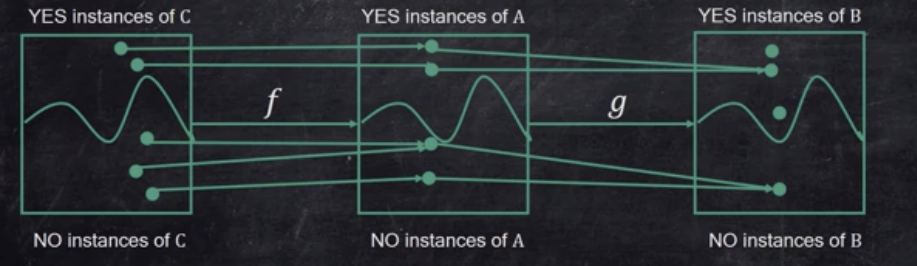
\includegraphics[width=0.5\textwidth]{fig/transitivity-reduction.png}
\end{figure}

In the example, each square represents all possible inputs to that problem and there is infinity many of them. There are some arbitrary unknown partitional inputs into those that are YES instances and those that are No instances. For examples, we draw those arbitrary curves within each of the rectangles. The points above are suppose to be the YES instances of the problem and the points below are the NO instances of the problem. 

Remember that reduction perverse the answer. So the fact that C is reduced to A means that some function $f$ which maps every point in the domain of C to the second box, which is instances of problem A while preserving the answer. Moreover, we just done reduction from A to B by function $g$, which is also answer-preserving.

Then let $x$ be any instance of $C$. $g(f(x))$ is an instance of $B$. Furthermore, $x$ is a YES instance if and only if $g(f(x))$ is a YES instance. So $g(f(x))$ looks like a reduction from $C$ to $B$. The composed function is actually poly-time because of the compositional properties of polynomials.

\subsection{Recipe For Proving a Problem NP-Complete}
To show problem $B$ is NP-complete,
\begin{itemize}
	\item First show $B \in \text{NP}$.
	\item Take a known NP-complete problem A.
	\item Construct a poly-time reduction from A to B.
	\item Prove that the reduction is poly-time and correct, i.e. maps YES instances of A to YES instances of B and NO instances of A to NO instances of B.
\end{itemize}

By transitivity of reductions, since we know all problems in NP reduce to A, we will have shown that all problems in NP reduce to B. So $B$ is NP-complete.











\section{Boolean Circuit Problem}
\subsection{Boolean Logic}
Since the first NP-completeness problem is proved in the context of boolean circuit, let's refresh some of the important concepts in this field.

Boolean variables: $x, y$ $\in$ $\{x| x \in \{0, 1\}\}$ or $\{x| x \in \{\text{T}, \text{F}\}\}$. Variables like $x$, $\bar{x}$ are called \textbf{literals}.

Operators: AND, OR, NOT. An operation of literals such as $(\bar{x} + y + z)$ is called a \textbf{clause}.

A formula in \textbf{conjunctive normal form (CNF)} is an AND of clauses. A CNF formula evaluates to 1 if and only if at least one literal in each clause is true.

Satisfiability is the problem of deciding whether a CNF formula is satisfiable. If a formula is satisfiable, the assignment of values to variables that makes formula true is a satisfying assignment.

Truth Table considers every possible value for each of the variables involving in the boolean expression and then describes what the value fo the boolean expression is for each set of the value.  

There are many properties that the boolean operations and variables satisfy.
Commutative, associative, distributive law.
\subsubsection{Imply}
\textbf{Implies} ($x \Rightarrow y$) is an important but confusing boolean operator. It means whenever $x$ is true, $y$ is true. The following is an example:
Suppose we have $P$, $Q$, $R$, $S$ four cases,
\begin{itemize}
	\item $P:$ Paris is the capital of France. (T)
	\item $Q:$ Most ants have 6 legs.  (T)
	\item $R:$ Rome is the capital of France. (F)
	\item $S:$ Most ants have 5 legs. (F)
\end{itemize}
The true/false is annotated after each statement based on the facts in our world.

It is safe to say $P \Rightarrow Q$ is true because $P$ is true and $Q$ is true. The imply can be explained as "If this is a world where Paris is the capital of France, then most of the ants have 6 legs". This implication works since both $P$ and $Q$ are true.

Hence, $P \Rightarrow S$ is not true because in this world where Paris is the capital of France, ants do not have 5 legs. This implication dose not work.

However, $R \Rightarrow Q$ and $R \Rightarrow S$ are both true. It is because $R$ is false in our world so you would say "in the world where Rome is the capital of France, most ants have 6 legs" or "most of ants have 5 legs". Either way is fine since the implication are not promising anything to our world.

So the true table of imply operation is as follows. Note that imply has the same true value as $\bar{x} \vee y$.

\begin{table}[H]
	\centering
	\begin{tabular}{|l|l|l|l|l|}
		\hline
		x & y & $x \Rightarrow y$ & $\bar{x}$ & $\bar{x} \vee y$ \\ \hline
		0 & 0 & 1                 & 1         & 1                \\ \hline
		0 & 1 & 1                 & 1         & 1                \\ \hline
		1 & 0 & 0                 & 0         & 0                \\ \hline
		1 & 1 & 1                 & 0         & 1                \\ \hline
	\end{tabular}
\end{table}

If we have implies at both direction, we get an equivalent.

\begin{table}[H]
	\centering
	\begin{tabular}{|l|l|l|l|l|}
		\hline
		x & y & $x \Rightarrow y$ & $y \Rightarrow x$ & $x \iff y$ \\ \hline
		0 & 0 & 1                 & 1                 & 1          \\ \hline
		0 & 1 & 1                 & 0                 & 0          \\ \hline
		1 & 0 & 0                 & 1                 & 0          \\ \hline
		1 & 1 & 1                 & 1                 & 1          \\ \hline
	\end{tabular}
\end{table}
\subsubsection{Converse}
The converse of $P \Rightarrow Q$ is $Q \Rightarrow P$. The converse does not have to be true even if the original statement is true. For example,
\begin{itemize}
	\item $P:$ It will rain this afternoon.
	\item $Q:$ The flower bed will get wet.
\end{itemize} 
Therefore, $P \Rightarrow Q$ means if it rains then the flowerbed will be wet. It is a true statement. However, the converse can be descried as if the flower bed is wet then it must because of the rain. So the converse statement is not necessarily true.


\subsubsection{Contrapositive}
Another course related example,
\begin{itemize}
	\item $P:$ In a given connected weighted graph, all the weights are distinct.
	\item $Q:$ The minimum spanning tree is unique.
\end{itemize}
It is possible to prove that $P \Rightarrow Q$ is true while $Q \Rightarrow P$ is actually false.

The contra-positive of $P \Rightarrow Q$ is $\neg Q \Rightarrow \neg P$. Contra positive statement is logically identical to the original statement.
\subsection{Boolean Circuit}
Boolean Circuit is a directed acyclic graph. There are types of nodes: input nodes, AND nodes, OR nodes, NOT nodes.
\begin{itemize}
	\item Input nodes have 0 in-degree
	\item AND nodes as well as OR nodes have in-degree 2.
	\item NOT nodes have in-degree 1.
\end{itemize}
No restriction on the out-degree for the nodes mentioned above. However, there is one special node designed as output node with out-degree 1. The value of the circuit is the value on the out-edge of the output node.
\subsubsection{Circuits as Computers}
Everything a computer does can be done by circuits, with a big caveat. Computers can compute on inputs of any length. Circuits are hardwired to handle only one length. So to simulate a computer, we need a family of circuits: one for each length of input. It is easy to see that a polynomial time algorithm on a computer can be simulated by a family of circuits, where the $n^{\text{th}}$ circuit has size (number of gates) polynomial in $n$.
\subsubsection{Circuit Value Problem}
In the circuit value problem, we are given a circuit and Boolean values for the input nodes. We need to compute the value of the circuit. This problem can be easily solved in polynomial time. Simply find the value of each node in topological sort order until we get the value of the output node. (Recall that circuit is a DAG.)
\begin{figure}[H]
	\centering
	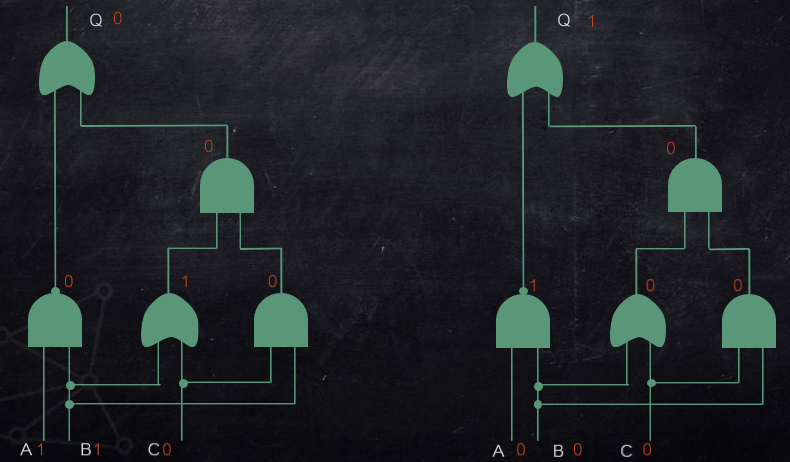
\includegraphics[width=0.5\textwidth]{fig/bool-logic.png}
\end{figure}
\subsubsection{Circuit Satisfiability Problem}
Circuit Satisfiability Problem is a famous NP-complete problem, where
\begin{itemize}
	\item Here the inputs are Boolean variables
	\begin{itemize}
		\item The inputs are not not specific boolean values, i.e. True, False
		\item The inputs are Boolean variables, i.e. $x_1$, $x_2$ etc.
	\end{itemize}
	\item We want to know if there exist values for the variables so that the circuit value evaluates to 1.
\end{itemize}

For example, for the above circuit plot, we would like to know if there is a set of $(A, B, C)$ so that the output of the circuit $Q$ equal to 1.
\section{Circuit Satisfiability is NP-Complete}
\subsection{Cook-Levin Theorem}
The theorem is often stated as:
\begin{theorem}
	Satisfiability is NP-complete.
\end{theorem}
\subsection{Circuit Satisfiability (CSAT)}
We will sketch the proof of a similar statement first:
\begin{theorem}
	Circuit satisfiability is NP-complete.
\end{theorem}

\begin{proof}
	Circuit satisfiability (CSAT) is easily seen to be in NP. A YES-instance of CSAT is a circuit whose input variables can be set to make the circuit evaluate to a 1. Given a YES-instance $c$ with $n$ input variables, a good certificate is an assignment of truth values to these input variables that cause $c$ to compute 1. A verifier only has to solve the circuit value problem that can be done in polynomial time.
	
	How do we reduce every problem in NP to CSAT? Let $B$ be any problem in NP. We will come up with a poly-time computable function $f$ mapping instances of $B$ to instances of CSAT, so that YES-instances map to YES-instances and NO-instances map to NO-instances.
	
	The key is that if we do it for any problem in NP without making assumptions about the problem, we would have shown reductions for all problems.
	
	So what do we know about any problem $B$ in NP? It has a poly-time verifier $V_B$. Remember that $V_B$ takes two inputs: an instance $x$ and a certificate $y$. The reduction $f$ that we construct will closely depend on $V_B$. $f$ must take as input an instance of $B$, say $x$, and convert it to an instance of CSAT, $f(x)$, with the answer-preserving of a reduction.
	
	Let us now examine the working of $V_B$ when dealing with instance $x$. $V_B$ takes $x$ and some certificate $y$ as inputs, and works as follows
	\begin{itemize}
		\item If $x$ is a YES-instance and $y$ is the right certificate, it accepts, i.e. it outputs 1.
		\item If $x$ is a NO-instance, for any certificate $y$, it rejects, i.e. it outputs 0.
	\end{itemize}

	Since $V_B$ runs in polynomial time, it can be converted to a poly-sized circuit with a number of inputs $= |x| + |y|$, which is polynomial in $|x|$. (Believable statement, but not fully proven here.) 
	
	Since we know the input $x$, the values for these inputs are set to match $x$. Since we do not know the input $y$, we leave the values for these inputs as Boolean variables. This is the circuit $f(x)$ which is the instance of CSAT created by our reduction. Note that the only inputs to $f(x)$ are the Boolean variables corresponding to the bits of $y$.
	
	There is a setting of the $y$ inputs that causes $f(x)$ to compute 1 if and only if $x$ is a YES-instance of B. So we have given a polynomial time reduction $f$ with the properties that 
	\begin{itemize}
		\item If $x$ is a YES-instance of B, then $f(x)$ is satisfiable.
		\item If $x$ in a NO-instance of B, then $f(x)$ is not satisfiable.
	\end{itemize}

	The reduction works from any problem $B$ in NP to CSAT. This proves that CSAT is NP-complete, and we have our first NP-complete problem.
\end{proof}

\subsection{Gates To Formulas}
\subsubsection{First Steps}
How do we write a formula (in CNF) to express that this gate is working correctly? Want to say $z = x \wedge y$ but ``='' is not a logical operator.

We can replace with $z \Leftrightarrow (x \wedge y)$, which is the same as $(z \Rightarrow (x \wedge y) \wedge ((x \wedge y) \Rightarrow z))$. Recall that $A \Rightarrow B$ is $\bar{A} \wedge B$. Using substitution, we can again rewrite as $(\bar{z} \vee (x \wedge y)) \vee (~\overline{(x \wedge y)} ~\vee z)$.

Using two rules of Boolean algebra: Distribution law for OR over AND, and De Morgan's law, we simplify to $(\bar{z} \vee x) \wedge (\bar{z} \vee y) \wedge (\bar{x} \vee \bar{y} \vee z)$.

\begin{itemize}
	\item Distribution law for OR over AND: $x \times (y + z) = (x \times y) + (x \times z)$
	\item De Morgan's law: $\overline{x \wedge y} = \bar{x} \vee \bar{y}$, $\overline{x \vee y} = \bar{x} \wedge \bar{y}$.
\end{itemize}

Check that the satisfying assignments of the last formula are all valid setting for the inputs and outputs of an AND gate. For example, if $x=0$ or $y=0$, then $z$ must be 0 to satisfy the first two clauses. But if both are 1, then $z$ must be 1 to satisfy the last clause.
\subsubsection{Using This Idea}
A similar derivation shows how to express that an OR gate is functioning correctly.

To convert a circuit into a formula, we introduce new variables on each of the internal wires of the circuit and tie the value of the output variable of a gate to the input variables using clauses as in the previous slide.




























\section{SAT is NP-complete}
\subsection{Satisfiability Decision Problem (SAT)}
Given a CNF furmula $\varphi(x_1, x_2, \cdots, x_n)$, is it satisfiable? The $x_i'$s are Boolean variables. Both the $x_i'$s and $\bar{x_i}'$s are literals, and both can occur in the formula $\varphi$.

YES-instance of SAT are formulas $\varphi$ that are satisfiable, and NO-instances are formulas that are not. If $\varphi$ is a YES-instance, it has a satisfying assignment. Given this assignment as certificate, a poly-time verifier can simply evaluate the formula and confirm that the result is 1. Thus SAT $\in$ NP.

\subsection{Proving SAT NP-complete}
We need to show a poly-time reduction from any problem in NP to SAT. Note that we already proved that CSAT NP-complete. So there are poly-time reductions from each problem in NP to CSAT. We also know (by transitivity of reductions) that if we can reduce CSAT to SAT, we would have shown that all problems in NP reduce to SAT.

When implement a reduction, we need to think about the input and the output of the reduction first. The input is an instance of the problem you are reducing from. In this case, the problem is CSAT. Therefore the input reduction is a circuit. The output reduction is an instance of SAT, which is a formula of a CNF. Given an instance (a circuit) $c$ of CSAT, we introduce a Boolean variable for the output wires of each gate and a Boolean variable for each input to C. 

In $\varphi = f(C)$, we write clauses expression that each gate is functioning correctly. It means $\varphi$ is satisfiable if and only if $C$ is satisfiable. If the overall output of $C$ is a wire labeled by variable $z$, in $\varphi$ we also add a clause consisting of just one literal: $z$. Note that in order to satisfy this last clause, $z$ must be 1.

In order to satisfy all the other clauses, the value of a variable at the output of any gate must follow logically from the values of the variables at the input to that gate. Thus, $\varphi$ can be satisfied if we can set the inputs to $C$, so that computes a 1.

The reduction is poly-time. We produce $O(1)$ clauses for each wire in the circuit, and since the circuit description must list all wires, the number of wires is linear in the input length. Thus the length of the formula produced is linear in the length of the circuit description.

As sketched, if $C$ is satisfiable, then $\varphi$ is satisfiable too. A satisfying assignment to $\varphi$ sets the variables corresponding to inputs of $C$ to the values in the satisfying assignment for $C$. It then sets the values for the variables at the wires of $C$ in a manner that is logically implied by the input setting. This will result in the output variable $z$ being set to 1, satisfying $\varphi$.

Conversely, if $C$ is not satisfiable, every setting of its input variable will cause $z$ to be 0. The only way to produce $z = 1$ is by making one of the gates behave erroneously. But the formula $\varphi$ is constructed in such a way that the erroneous operations of any gate will cause $\varphi$ to be false. Thus there will also be no satisfying assignment for $\varphi$. This complete the proof that SAT is NP-complete.

\subsection{3-SAT}
We can go a step further, say a formula $\varphi$ is a 3-CNF formula if it is a CNF formula with exactly 3 literals in each clause. By a reduction from SAT, we can show $3-SAT$ is NP-complete. $3-SAT$ turns out to be the fountainhead from which proofs of NP-completeness of many diverse problems flow.



















\section{Independent Set is NP-complete}
\subsection{Independent Set (IS)}
Given a graph $G= (V, E)$, an independent set is a subset $S \subseteq V$ such that for any two vertices $u, v \in S$, there is no edge between $u$ and $v$.

The independent set decision problem (IS):
\begin{itemize}
	\item Instance: graph $G$ and number $K$
	\item Question: does $G$ have an independent set of size $K$?
\end{itemize}

Clearly, this is a NP problem. The certificate is just the $K$ vertices that form an independent set.

\subsection{Independent Set is NP-Compelete}

We show that 3-SAT reduces to Independent Set. 

\subsubsection{Main Idea}
The reduction maps literals into nodes of a graph, with the idea that a set of true literals will form an independent set.

\begin{itemize}
	\item Problem: in a YES-instance of 3-SAT, we can have one, two, or three literals true in each clause. So we do not get a definite size for the independent set.
	\item Solution: ensure that at most  one true literal in each clause can be part of the independent set, by connecting the 3 literals of the clause by a triangle.
\end{itemize}

Now, set the target size of the independent set to be $m$, the number of clauses. Only way to get to target is to pick exactly one literal from every clause. Since these literals have to be non-conflicting (to make an independent set), they can be simultaneously set to true, proving that the formula is satisfiable.

Let $\phi = \wedge_{i=1}^m C_i$, the $i$-th clause, is equal to $(\ell_1^i + \ell_2^i + \ell_3^i)$. The reduction $f$ transforms $\varphi$ into a graph $G$ and a number $K$ such that $\varphi$ is satisfiable if and only if $f(\varphi)$ is a YES-instance of Independent Set.

It seems mysterious that we can transform a logic problem into a graph problem. The main idea is to remember that to make $\varphi$ true, we must make at least 1 literal true in each clause. Also, rules of Boolean logic say we cannot choose to make $x$ true in one clause and $\bar{x}$ true in another; these are conflicting literals that cannot both be true.

Even though a satisfying assignment could make more than one literal true, we convert the clause into a triangle where an independent set can pick just one vertex. If two clauses have conflicting literals, we draw an edge between the corresponding nodes. Thus, an independent set can never pick nodes corresponding to conflicting literals. We now set $K = m$ and ask if $G$ has an independent set of size $K$.

\begin{figure}[H]
	\centering
	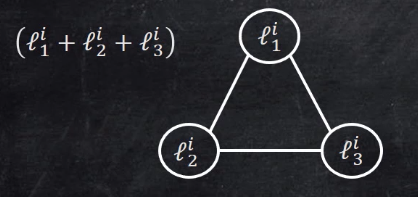
\includegraphics[width=0.3\textwidth]{fig/3-literal.png}	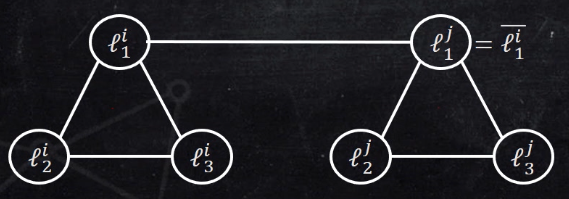
\includegraphics[width=0.4\textwidth]{fig/converse-literal.png}
\end{figure}

\subsubsection{Proof of Correctness}
If $\varphi$ is satisfiable:
\begin{itemize}
	\item In the satisfying assignment, we can find one literal per clause that is true.
	\item Since these literal are simultaneously true, there cannot be conflicting literals among them.
	\item In the graph, there are $m$ nodes corresponding to these literals, one per clause triangle.
	\item These $m$ nodes from an independent set (no edges due to conflicts), hence we have created a YES-instance of independent set.
\end{itemize}
 
Conversely, suppose $G$ is a YES-instance of IS:
\begin{itemize}
	\item Let $S$ be the subset of $m$ nodes that forms an independent set.
	\item Clearly, $S$ contains one node from each clause, and it contains no conflicting literals.
	\item Making all the literals corresponding to $S$ true causes $\varphi$ to be true.
	\item Thus we must have started with a YES-instance of 3-SAT.
\end{itemize}
 
\subsection{Points to Note}

To prove a reduction from $A$ to $B$ correct, we have to prove YES-instances of $A$ map to YES-instance of $B$ and NO-instances of $A$ map to NO-instances of $B$.

It is often convenient to do the second part by proving the equivalent contra-positive statement: \textbf{If the instance of $B$ created by the reduction is a YES-instance, it must have come from a YES-instance of $A$.}  
 
A reduction from $A$ to $B$ is a function whose domain is the instances of $A$. So it must be defined on ``all''  instances of $A$. However, it does not have to be one-to-one or onto, so not all instances of $B$ might be in the image of the reduction.
 
 
 
 
 
 
 
 
 
 
 
 
 
 
 
 
 
 
 
 
\section{3-Coloring is NP-Complete}
\subsection{Graph Coloring}
Given a graph $G = (V, E)$, a valid coloring is an assignment of colors to the vertices, so that if $u$ and $v$ are adjacent then they get different colors.

Graph 3-coloring decision problem (3-COL):
\begin{itemize}
	\item Instance: graph $G$.
	\item Question: Is there a valid coloring of $G$ with 3 colors?
\end{itemize}

Clearly in NP. The certificate is just the colors assigned to each vertex. An algorithm can check in polynomial time that only 3 colors are being used, and that adjacent vertices have different colors.

\subsection{3-COL is NP-complete}
We now have a choice of which NP-complete problem to reduce to 3-COL. It turns of 3-SAT is still the right one!

Let $\varphi = \wedge_{i=1}^m C_i$ where $C_i$, the $i$-th clause, is equal to $(l_1^i \vee l_2^i \vee l_3^i)$. The reduction $f$ transforms $\varphi$ into a graph $G$ such that $\varphi$ is satisfiable if and only if $f(\varphi)$ is 3-colorable.

Recall that to make $\varphi$ true, we must make at least 1 literal true in each clause. Then we may consider:
\begin{itemize}
	\item How do we relate the truth values of variables to colors in a graph?
	\item How do we ensure that if $x$ is assigned to TRUE, then $\bar{x}$ is assigned to FALSE (and vice versa)?
	\item How do we translate a clause being satisifiable to some portion of the graph being colorable?
\end{itemize}
\subsubsection{Relating Truth Values To Colors}
Add a triangle on 3 vertices $a$, $b$ and $c$ (called the ``reference triangle'') to the graph. In any valid coloring, $a$, $b$ and $c$ must be colored using all 3 colors. Arbitrarily designate $a$'s color TRUE, $b$'s color FALSE, and $c$'s color to be RED. Make nodes for each pair of literals $x_i$ and $\bar{x_i}$. 

How do we ensure that exactly one of these will be colored TRUE, the other colored FALSE, and neither colored RED? The Answer is simple, make $x_i$ and $\bar{x_i}$ adjacent to each other and to $c$.

\begin{figure}[H]
	\centering
	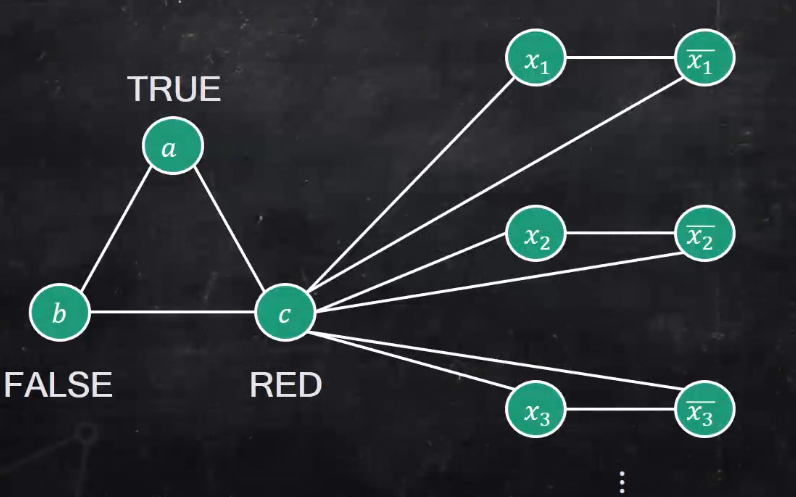
\includegraphics[width=0.5\textwidth]{fig/3-col.png}
\end{figure}

Now let's add more constrain on the graph for the clauses. Consider a clause like $(x \vee y \vee z)$. We already have nodes for $x$, $y$ and $z$ (each of which is forced to be colored TRUE or FALSE). We connect them by a nice ``OR'' gadget as follow:

\begin{figure}[H]
	\centering
	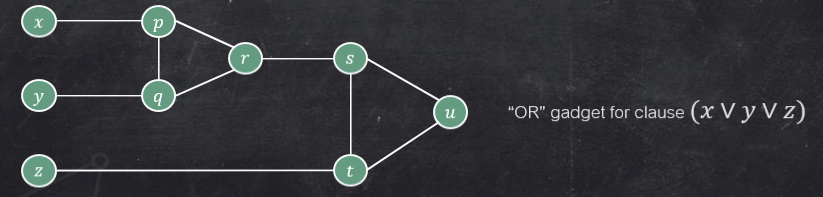
\includegraphics[width=0.7\textwidth]{fig/3-col-or-gadget.png}
\end{figure}

It can be checked the if at least one of $x$, $y$ and $z$ is colored TRUE, then $u$ can be colored TRUE. Otherwise, if all 3 of $x$, $y$ and $z$ are colored FALSE, $u$ must be colored FALSE.

For each clause, add this gadget to the graph using distinct nodes, except for the literal nodes shared between all clauses. Note that, each gadget has its own $p$, $q$, $r$, $s$ $t$ and $u$. For example,

\begin{figure}[H]
	\centering
	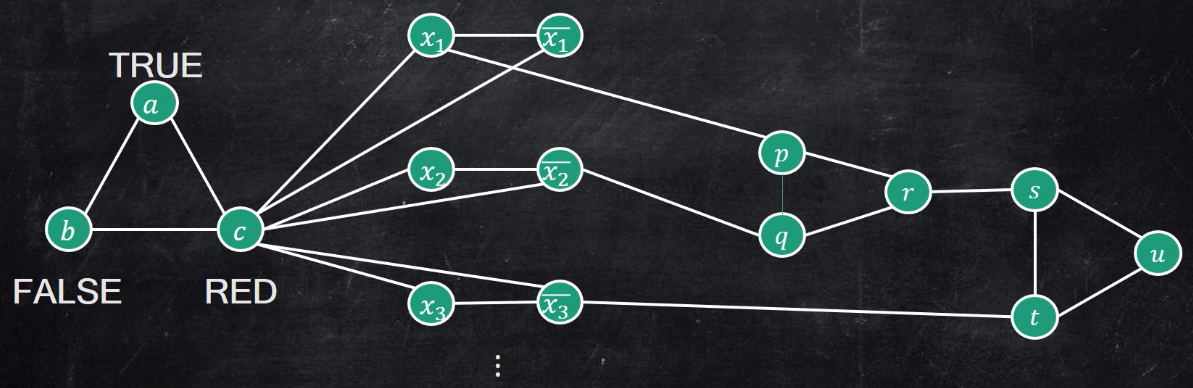
\includegraphics[width=0.7\textwidth]{fig/3-col-or-gadget-in-graph.png}
\end{figure}

To finish off the construction, connect the node at the tip of each clause gadget (labeled $u$ in our example figure) to node $b$ and $c$ in the reference triangle, whose colors are FALSE and RED respectively. In order for this graph to be 3-colorable, we are forced to color the node at the tip of each clause gadget ($u$) TRUE. This is only possible if one of the literals input to the clause is TRUE.

\subsubsection{Proving Correctness}
Our intuition built up in constructing the reduction translates easily into a correctness proof.

Suppose we  start with a YES-instance, $\varphi$ of 3-SAT, use a satisfying assignment to decide which literal in each pair to color ``True'' (the color of $a$ in the reference triangle) and which one to color ``FALSE'' (the color of $b$). Now complete the coloring-assignment by coloring each clause gadget so that node $u$ at the tip of each gadget has color TRUE. This shows we have create a YES-instance of 3-COL!

Conversely, if the reduction created a YES-instance of 3-COL, then look at a valid coloring and treat as true all the literals colored the same as $a$. This sets at least one literal true in each clause. Otherwise we wouldn't have been able to color the clause gadget.

\subsubsection{Wrapping Up}
Reduction is easily computed in polynomial time. When constructing a reduction, remember these points:
\begin{itemize}
	\item Reduce from known NP-complete problem to problem you want to prove NP-complete. Getting the direction of the reduction wrong is a common but serious error.
	\item Do not try to ``solve'' either problem. It's unlikely that you can do it correctly and efficiently.
	\item Instead, do the reduction without knowing whether the instance you are transforming is a YES-instance or a NO-instance.
\end{itemize}

\subsubsection{Motivation}
Graph coloring is an important problem.

``Interference graphs'' are graphs where every node is a task, person, or entity, and edges denote tasks that interfere with one another or people who do not get along. A valid coloring is a way of assigning ``slots'' to these entities so that interfering entities get different slots. Example applications include: compilers allocating variables to registers, allocating frequencies to radio stations, people to tasks, etc.

The bad news is that we have just shown that finding the best solution is unlikely to be efficient.  We must resort to heuristics, or restrict the type of graph. We have already seen one example of the latter: activity selection.


































\section{Vertex Cover is NP-Complete}
\subsection{Vertex Cover (VC)}
Given a graph $G=(V,E)$, a vertex cover is a subset $S \subseteq V$, so that for each edge $(u,v) \in E$ at least one of $u$ or $v$ lies in $S$.

Vertex cover decision problem (VC):
\begin{itemize} 
	\item Instance: graph $G$, integer $k$
	\item Question: does $G$ have a vertex cover of size at most $k$?
\end{itemize}

Clearly in NP. The certificate is just the subset of vertices forming the vertex cover. An algorithm can check in polynomial time that the subset is of the right size and that every edge is covered.

\subsection{IS and VC}
Once again, we have a choice of which NP-complete problem to reduce to VC. This time independent set (IS) is the right one. Before we do the reduction, let's understand the relationship between IS and VC. The following example shows that $(V-S)$ is a vertex cover, where $S$ is an independent set. This also holds true in the other direction: if $S$ is a vertex cover then $V-S$ is an independent set.

\begin{figure}[H]
	\centering
	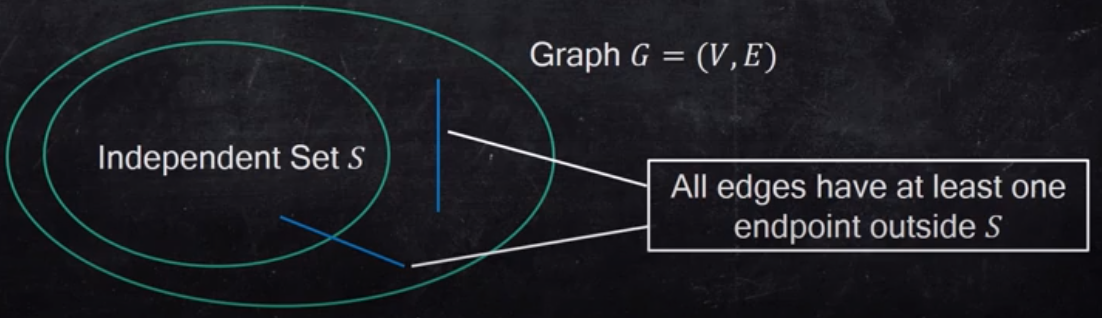
\includegraphics[width=0.5\textwidth]{fig/is-vc.png}
\end{figure}

Thus, a graph with n vertices has an independent set of size at least $k$ if and only if it has a vertex cover of size at most $n-k$.

The reduction is now fairly obvious: Given an instance $\langle G, k \rangle$ of IS, we transform it into an instance $\langle G,n-k \rangle$ of VC.

\subsubsection{Reduction}
If $G$ has an IS, $S$, of size at least $k$, then $V-S$ is a VC of size at most $n-k$. Thus, YES-instances of IS map to YES-instances of VC. If $G$ has a VC, S, of size at most $n-k$, then it has an IS, $V-S$, of size at least $k$. Thus, YES instances of VC map to YES instances of IS. It's easy to see that the reduction runs in poly-time since we are only changing the number.



\section{Clique is NP-complete}
A clique in $G=(V,E)$ is a subset $S$ of vertices such that $\forall x,y \in S, (x,y) \in E$.

Clique decision problem:
\begin{itemize}
	\item Instance: graph $G=(V, E)$ and a number $k$
	\item Question: does $G$ contain a clique of size at least $k$?
\end{itemize}

CLIQUE is NP-complete: reduction from IS.

Main idea: the complement $G^c=(V,E^c)$ of a graph $G=(V,E)$ is a graph on the same vertex set, where $(u,v) \in E^c \iff (u,v) \notin E$. Non-edges of G become edges of $G^c$ and vice versa. Note that any set of vertices that forms an IS in $G$ forms a clique in $G^C$ and vice verse.

\subsubsection{Reduction and Proof}
Reduction from IS: Given instance $\langle G,k \rangle$ of IS, transform it into instance $\langle G^c,k \rangle$ of CLIQUE.

Easy proof of correctness:

If $\langle G, k\rangle$ is a YES-instance of IS, then it has an independent set $S$ of size $k$. $S$ is a clique of size $k$ in $G^C$. Thus $\langle G^C, k \rangle$ is a YES-instance of CLIQUE. 

Conversely, if the instance $\langle G, k\rangle$ is created by the reduction is a YES instance of CLIQUE, then the instance we started from $\langle G, k \rangle$, must be a YES-instance of IS.

Running Time: Complementing a graph requires $O(n^2)$ times.









































\section{Subset-sum is NP-complete}
\subsection{Subset-sum}
Subset sum decision problem:
\begin{itemize}
	\item Instance: $n$ numbers $a_1, a_2, \cdots, a_n$ and a target $T$.
	\item Question: is there a subset $S$ of the indices such that $\sum_{i \in S} a_i = T$.
\end{itemize}

subset sum problem is in NP. Suppose you are given a YES-instance $\langle (a_1, a_2, \cdots, a_n), T \rangle$. Then a certificate showing it is a YES-instance would be that subset of numbers which add up to $T$. We could check the certificate by adding up $(a_1, a_2, \cdots, a_n)$ to see if the sum is $T$.

We prove that subset sum is NP-complete by a complicated reduction from 3-SAT. Let $\varphi$ be a 3-SAT instance with $n$ variables and $m$ clauses. We create a subset sum instance with $2n + 2m$ numbers, each with $n+m$ digits!

Every row suppose to be one number. The first a few digits are the variable columns and the last few digits are the clauses columns. So there are $n + m$ columns in total. 

\begin{figure}[H]
	\centering
	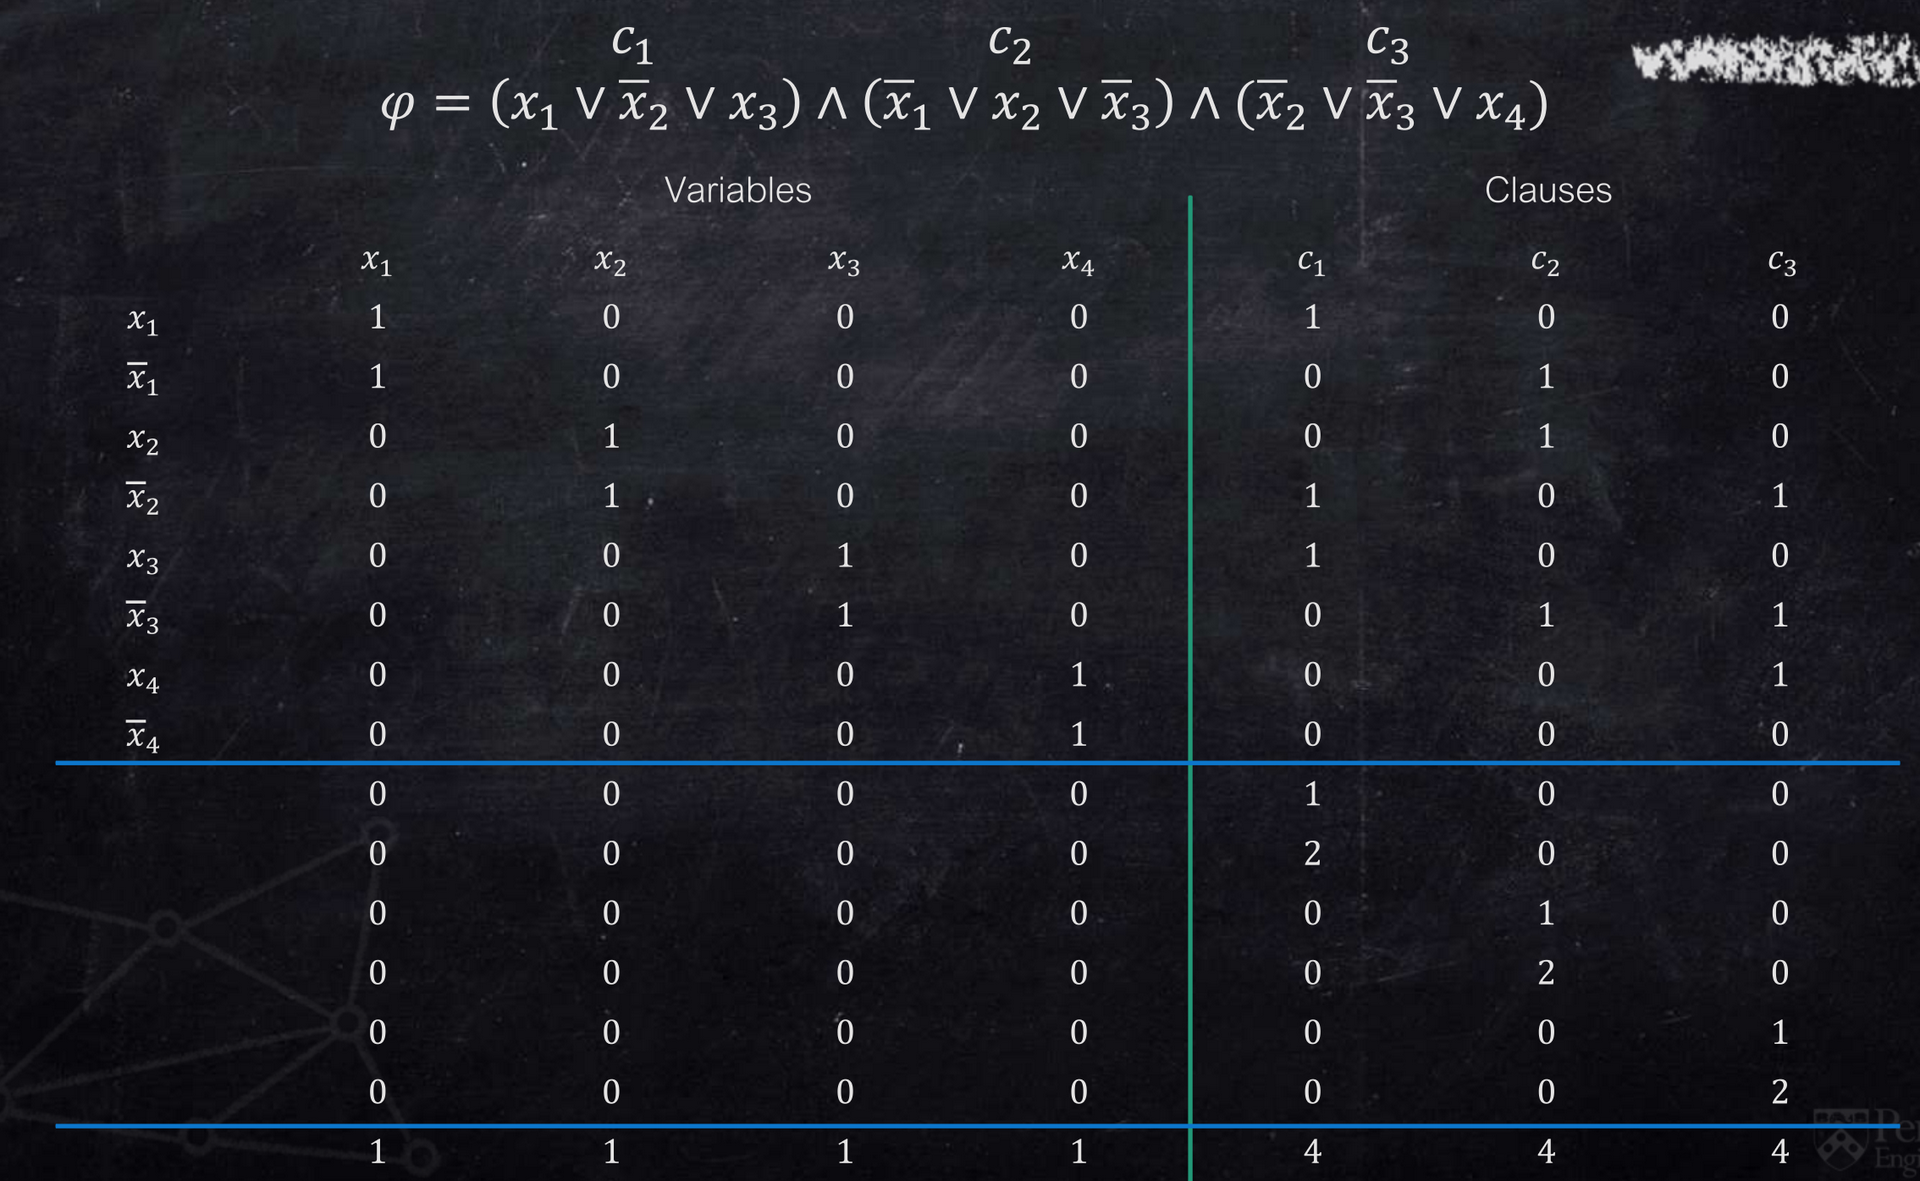
\includegraphics[width=0.5\textwidth]{fig/subset-sum.png}	
\end{figure}

In general,
\begin{figure}[H]
	\centering
	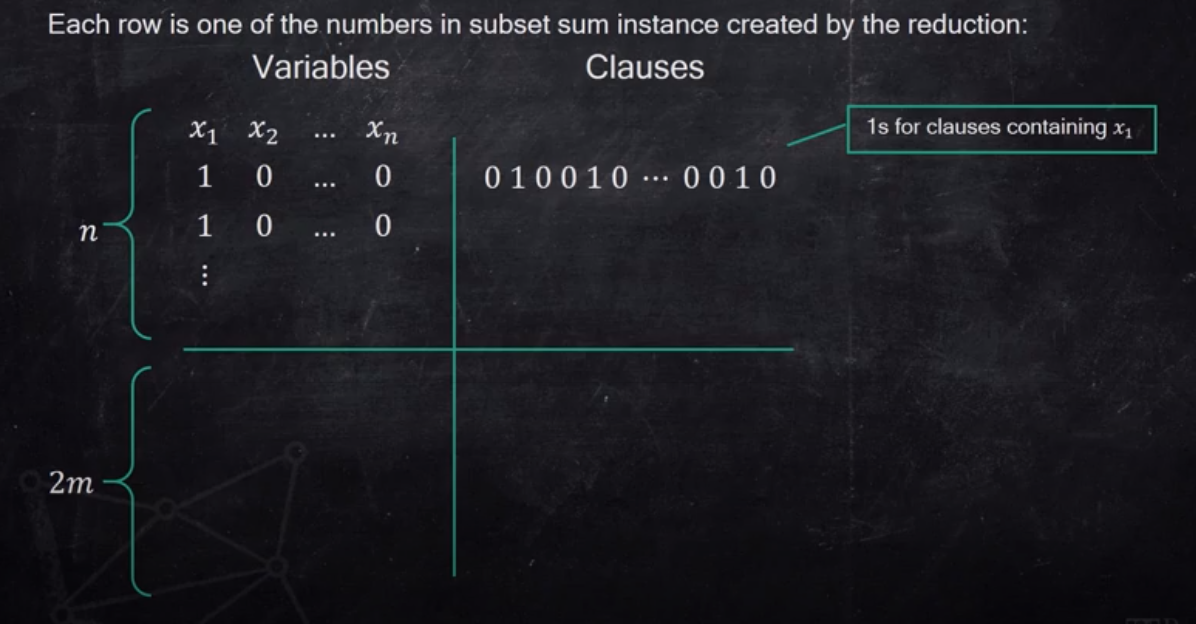
\includegraphics[width=0.5\textwidth]{fig/subset-sum-general.png}	
\end{figure}

\subsubsection{Proof of Correcness}
Suppose $\varphi$ is satisfiable. Let $a$ be a satisfying assignment for $\varphi$. Pick the numbers corresponding to the true literals in $a$. In the variable columns, we have picked one 1 per column, so the target is met. In any clause column, we have picked at least one 1 from the upper half but may have picked up to three 1s (if all 3 literals in the clause are true). Then we can get to the target of 4 by picking one or both numbers from lower half that have non-zero entries for that column. So, we have created a YES instance of subset sum.

If we have created a YES instance of subset-sum, look at the subset of numbers that add up to the target. Note that we only consider the YES-instance constructed by algorithm instead of any YES-instance.

For each variable $x_i$, this subset must have exactly one of the two numbers corresponding to $x_i$ or $(\bar{x_i})$. Treat the literal corresponding to the chosen number as TRUE. Then in each clause column, the chosen numbers (true literals) must contribute at least 1, otherwise we couldn't get to the target of 4 or these columns. Thus, the assignment we have constructed is a satisfying assignment for $\varphi$. Thus, $\varphi$ must be a YES instance of 3-SAT.

\end{document}






















